% -- Generated using the code: draw_clocks(v1=-0.1, v2=0.4, tstart=-1, tend=7,)
% -- -> moving_clocks_single_fig(-0.1, 0.4, -1, 7, -0.5) is slightly off



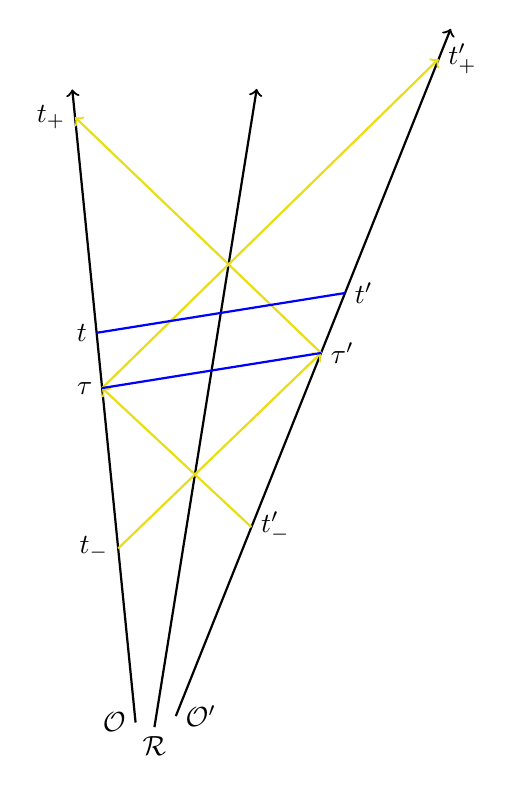
\begin{tikzpicture}
    % Draw lines of observers
    \draw[->, thick] (-0.40201512610368484, -0.9547859244962514) -- (-1.2060453783110547, 7.0855165975774455);
    \draw[->, thick] (0.10910894511799615, -0.8728715609439694) -- (3.600595188893874, 7.855844048495725);
    \draw[->, thick] (-0.1623618057543558, -1.0130949392667081) -- (1.1365326402804907, 7.091664574866957);

    % Draw trajectories of light
    \draw[->, thick, black!10!yellow] (-0.6231234454607115, 1.256297269074015) -- (1.9537009395844693, 3.7386084252222127);
    \draw[->, thick, black!10!yellow] (1.9537009395844693, 3.7386084252222127) -- (-1.1707397509030126, 6.732460323497025);
    \draw[->, thick, black!10!yellow] (1.0692676621563626, 1.5275252316519465) -- (-0.8267934763476378, 3.292997577943277);
    \draw[->, thick, black!10!yellow] (-0.8267934763476378, 3.292997577943277) -- (3.4472811660885947, 7.472558991482527);

    % Draw lines of simultaneity
    \draw[thick, blue] (-0.8969315981818621, 3.9943787962855204) -- (2.2582744141224786, 4.500042111567237);
    \draw[thick, blue] (-0.8267934763476378, 3.292997577943277) -- (1.9537009395844693, 3.7386084252222127);

    % Make labels
    \draw (-0.40201512610368484, -0.9547859244962514) node[left] {$\mathcal{O}$};
    \draw (-0.6231234454607115, 1.256297269074015) node[left] {$t_-$};
    \draw (-1.1707397509030126, 6.732460323497025) node[left] {$t_+$};
    \draw (1.9537009395844693, 3.7386084252222127) node[right] {$\tau'$};
    \draw (2.2582744141224786, 4.500042111567237) node[right] {$t'$};
    \draw (0.10910894511799615, -0.8728715609439694) node[right] {$\mathcal{O}'$};
    \draw (1.0692676621563626, 1.5275252316519465) node[right] {$t'_-$};
    \draw (3.4472811660885947, 7.472558991482527) node[right] {$t'_+$};
    \draw (-0.8267934763476378, 3.292997577943277) node[left] {$\tau$};
    \draw (-0.8969315981818621, 3.9943787962855204) node[left] {$t$};
    \draw (-0.1623618057543558, -1.0130949392667081) node[below] {$\mathcal{R}$};
\end{tikzpicture}